% Options for packages loaded elsewhere
\PassOptionsToPackage{unicode}{hyperref}
\PassOptionsToPackage{hyphens}{url}
%
\documentclass[
  man, donotrepeattitle,floatsintext]{apa6}
\usepackage{amsmath,amssymb}
\usepackage{lmodern}
\usepackage{iftex}
\ifPDFTeX
  \usepackage[T1]{fontenc}
  \usepackage[utf8]{inputenc}
  \usepackage{textcomp} % provide euro and other symbols
\else % if luatex or xetex
  \usepackage{unicode-math}
  \defaultfontfeatures{Scale=MatchLowercase}
  \defaultfontfeatures[\rmfamily]{Ligatures=TeX,Scale=1}
\fi
% Use upquote if available, for straight quotes in verbatim environments
\IfFileExists{upquote.sty}{\usepackage{upquote}}{}
\IfFileExists{microtype.sty}{% use microtype if available
  \usepackage[]{microtype}
  \UseMicrotypeSet[protrusion]{basicmath} % disable protrusion for tt fonts
}{}
\makeatletter
\@ifundefined{KOMAClassName}{% if non-KOMA class
  \IfFileExists{parskip.sty}{%
    \usepackage{parskip}
  }{% else
    \setlength{\parindent}{0pt}
    \setlength{\parskip}{6pt plus 2pt minus 1pt}}
}{% if KOMA class
  \KOMAoptions{parskip=half}}
\makeatother
\usepackage{xcolor}
\IfFileExists{xurl.sty}{\usepackage{xurl}}{} % add URL line breaks if available
\IfFileExists{bookmark.sty}{\usepackage{bookmark}}{\usepackage{hyperref}}
\hypersetup{
  pdftitle={Re-analysing the data from Moffatt et al. (2020): What can we learn from an under-powered absence of difference?},
  pdfauthor={Ladislas Nalborczyk1, 2, 3},
  pdflang={en-EN},
  pdfkeywords={NHST, Bayes factor, reanalysis, inner speech, rumination, electromyography},
  hidelinks,
  pdfcreator={LaTeX via pandoc}}
\urlstyle{same} % disable monospaced font for URLs
\usepackage{graphicx}
\makeatletter
\def\maxwidth{\ifdim\Gin@nat@width>\linewidth\linewidth\else\Gin@nat@width\fi}
\def\maxheight{\ifdim\Gin@nat@height>\textheight\textheight\else\Gin@nat@height\fi}
\makeatother
% Scale images if necessary, so that they will not overflow the page
% margins by default, and it is still possible to overwrite the defaults
% using explicit options in \includegraphics[width, height, ...]{}
\setkeys{Gin}{width=\maxwidth,height=\maxheight,keepaspectratio}
% Set default figure placement to htbp
\makeatletter
\def\fps@figure{htbp}
\makeatother
\setlength{\emergencystretch}{3em} % prevent overfull lines
\providecommand{\tightlist}{%
  \setlength{\itemsep}{0pt}\setlength{\parskip}{0pt}}
\setcounter{secnumdepth}{-\maxdimen} % remove section numbering
% Make \paragraph and \subparagraph free-standing
\ifx\paragraph\undefined\else
  \let\oldparagraph\paragraph
  \renewcommand{\paragraph}[1]{\oldparagraph{#1}\mbox{}}
\fi
\ifx\subparagraph\undefined\else
  \let\oldsubparagraph\subparagraph
  \renewcommand{\subparagraph}[1]{\oldsubparagraph{#1}\mbox{}}
\fi
\newlength{\cslhangindent}
\setlength{\cslhangindent}{1.5em}
\newlength{\csllabelwidth}
\setlength{\csllabelwidth}{3em}
\newlength{\cslentryspacingunit} % times entry-spacing
\setlength{\cslentryspacingunit}{\parskip}
\newenvironment{CSLReferences}[2] % #1 hanging-ident, #2 entry spacing
 {% don't indent paragraphs
  \setlength{\parindent}{0pt}
  % turn on hanging indent if param 1 is 1
  \ifodd #1
  \let\oldpar\par
  \def\par{\hangindent=\cslhangindent\oldpar}
  \fi
  % set entry spacing
  \setlength{\parskip}{#2\cslentryspacingunit}
 }%
 {}
\usepackage{calc}
\newcommand{\CSLBlock}[1]{#1\hfill\break}
\newcommand{\CSLLeftMargin}[1]{\parbox[t]{\csllabelwidth}{#1}}
\newcommand{\CSLRightInline}[1]{\parbox[t]{\linewidth - \csllabelwidth}{#1}\break}
\newcommand{\CSLIndent}[1]{\hspace{\cslhangindent}#1}
\ifLuaTeX
\usepackage[bidi=basic]{babel}
\else
\usepackage[bidi=default]{babel}
\fi
\babelprovide[main,import]{english}
% get rid of language-specific shorthands (see #6817):
\let\LanguageShortHands\languageshorthands
\def\languageshorthands#1{}
% Manuscript styling
\usepackage{upgreek}
\captionsetup{font=singlespacing,justification=justified}

% Table formatting
\usepackage{longtable}
\usepackage{lscape}
% \usepackage[counterclockwise]{rotating}   % Landscape page setup for large tables
\usepackage{multirow}		% Table styling
\usepackage{tabularx}		% Control Column width
\usepackage[flushleft]{threeparttable}	% Allows for three part tables with a specified notes section
\usepackage{threeparttablex}            % Lets threeparttable work with longtable

% Create new environments so endfloat can handle them
% \newenvironment{ltable}
%   {\begin{landscape}\begin{center}\begin{threeparttable}}
%   {\end{threeparttable}\end{center}\end{landscape}}
\newenvironment{lltable}{\begin{landscape}\begin{center}\begin{ThreePartTable}}{\end{ThreePartTable}\end{center}\end{landscape}}

% Enables adjusting longtable caption width to table width
% Solution found at http://golatex.de/longtable-mit-caption-so-breit-wie-die-tabelle-t15767.html
\makeatletter
\newcommand\LastLTentrywidth{1em}
\newlength\longtablewidth
\setlength{\longtablewidth}{1in}
\newcommand{\getlongtablewidth}{\begingroup \ifcsname LT@\roman{LT@tables}\endcsname \global\longtablewidth=0pt \renewcommand{\LT@entry}[2]{\global\advance\longtablewidth by ##2\relax\gdef\LastLTentrywidth{##2}}\@nameuse{LT@\roman{LT@tables}} \fi \endgroup}

% \setlength{\parindent}{0.5in}
% \setlength{\parskip}{0pt plus 0pt minus 0pt}

% Overwrite redefinition of paragraph and subparagraph by the default LaTeX template
% See https://github.com/crsh/papaja/issues/292
\makeatletter
\renewcommand{\paragraph}{\@startsection{paragraph}{4}{\parindent}%
  {0\baselineskip \@plus 0.2ex \@minus 0.2ex}%
  {-1em}%
  {\normalfont\normalsize\bfseries\itshape\typesectitle}}

\renewcommand{\subparagraph}[1]{\@startsection{subparagraph}{5}{1em}%
  {0\baselineskip \@plus 0.2ex \@minus 0.2ex}%
  {-\z@\relax}%
  {\normalfont\normalsize\itshape\hspace{\parindent}{#1}\textit{\addperi}}{\relax}}
\makeatother

% \usepackage{etoolbox}
\makeatletter
\patchcmd{\HyOrg@maketitle}
  {\section{\normalfont\normalsize\abstractname}}
  {\section*{\normalfont\normalsize\abstractname}}
  {}{\typeout{Failed to patch abstract.}}
\patchcmd{\HyOrg@maketitle}
  {\section{\protect\normalfont{\@title}}}
  {\section*{\protect\normalfont{\@title}}}
  {}{\typeout{Failed to patch title.}}
\makeatother

\usepackage{xpatch}
\makeatletter
\xapptocmd\appendix
  {\xapptocmd\section
    {\addcontentsline{toc}{section}{\appendixname\ifoneappendix\else~\theappendix\fi\\: #1}}
    {}{\InnerPatchFailed}%
  }
{}{\PatchFailed}
\keywords{NHST, Bayes factor, reanalysis, inner speech, rumination, electromyography\newline\indent Word count: 3152 (excluding abstract, references, tables, and figures)}
\usepackage{lineno}

\linenumbers
\usepackage{csquotes}
\ifLuaTeX
  \usepackage{selnolig}  % disable illegal ligatures
\fi

\title{Re-analysing the data from Moffatt et al. (\protect\hyperlink{ref-moffatt_inner_2020}{2020}): What can we learn from an under-powered absence of difference?}
\author{Ladislas Nalborczyk\textsuperscript{1, 2, 3}}
\date{}


\shorttitle{The absence of evidence fallacy}

\authornote{

Correspondence concerning this article should be addressed to Ladislas Nalborczyk, LPC, CNRS, Aix-Marseille University, 13 Boulevard Gustave Desplaces, 13003 Marseille, France. E-mail: \href{mailto:ladislas.nalborczyk@univ-amu.fr}{\nolinkurl{ladislas.nalborczyk@univ-amu.fr}}

}

\affiliation{\vspace{0.5cm}\textsuperscript{1} Univ. Grenoble Alpes, CNRS, Grenoble INP, GIPSA-lab, 38000 Grenoble, France\\\textsuperscript{2} Aix Marseille Univ, CNRS, LPC, Marseille, France\\\textsuperscript{3} Aix Marseille Univ, CNRS, LNC, Marseille, France}

\abstract{%
Moffatt et al. (\protect\hyperlink{ref-moffatt_inner_2020}{2020}) reported the results of an experiment (N = 26 in the final sample) comparing the facial electromyographic correlates of mental rumination and distraction, following an experimentally induced stressor. Based on the absence of significant difference (and BFs between 3.6 and 4.3) in the perioral muscular activity between the rumination and distraction conditions, Moffatt et al. (\protect\hyperlink{ref-moffatt_inner_2020}{2020}) concluded that \emph{self-reported} inner experience was unrelated to peripheral muscular activity as assessed using surface electromyography. In this short commlentary, we show that there is limited evidence for the main conclusion put forward by Moffatt et al. (\protect\hyperlink{ref-moffatt_inner_2020}{2020}), and we suggest ways forward, both from a theoretical and a methodological perspective. Complete source code, reproducible analyses, and figures are available at \url{https://osf.io/ba3gk/}.
}



\begin{document}
\maketitle

\hypertarget{introduction}{%
\section{Introduction}\label{introduction}}

The activity of silently talking to oneself or ``inner speech'' is a foundational ability, allowing oneself to remember, plan, self-motivate, or self-regulate (for reviews, see \protect\hyperlink{ref-alderson-day_inner_2015}{Alderson-Day \& Fernyhough, 2015}; \protect\hyperlink{ref-loevenbruck_cognitive_2018}{Lœvenbruck et al., 2018}; \protect\hyperlink{ref-perrone-bertolotti_what_2014}{Perrone-Bertolotti et al., 2014}). However, whereas the use of inner speech is associated with many adaptive functions in everyday life, inner speech dysfunctions can be identified in multiple psychological disorders. For instance, rumination, broadly defined as unconstructive repetitive thinking about past events and current mood states (\protect\hyperlink{ref-Martin}{Martin \& Tesser, 1996}), is involved in the onset and maintenance of serious mental disorders such as depression, anxiety, eating disorders, or substance abuse (for review, see \protect\hyperlink{ref-Nolen-Hoeksema2008}{Nolen-Hoeksema et al., 2008}).

Given the predominantly verbal nature of rumination (e.g., \protect\hyperlink{ref-ehring_repetitive_2008}{Ehring \& Watkins, 2008}; \protect\hyperlink{ref-goldwin_concreteness_2013}{Goldwin et al., 2013}; \protect\hyperlink{ref-goldwin_concreteness_2012}{Goldwin \& Behar, 2012}; \protect\hyperlink{ref-mclaughlin_effects_2007}{McLaughlin et al., 2007}), we previously proposed to consider rumination as a form of inner speech and to study it using the methods that have historically been used to study other forms of inner speech, namely, by using surface electromyography (EMG) and motor interference protocols (e.g., \protect\hyperlink{ref-nalborczyk_dissociating_2021}{Nalborczyk, Banjac, et al., 2021}; \protect\hyperlink{ref-nalborczyk_articulatory_2022}{Nalborczyk et al., 2022}, \protect\hyperlink{ref-nalborczyk_orofacial_2017}{2017}; \protect\hyperlink{ref-nalborczyk_understanding_2019}{Nalborczyk, 2019}). We first showed that induced rumination was accompanied by increased facial (both over a forehead and a perioral site) muscular activity in comparison to a rest period (\protect\hyperlink{ref-nalborczyk_orofacial_2017}{Nalborczyk et al., 2017}). However, because rumination was only compared to a rest period, it remained uncertain whether this perioral activity was specifically related to (inner) speech processes. Therefore, we ran a follow-up study comparing verbal to non-verbal rumination, which suggested that the facial EMG correlates we had previously identified were not specifically related to the verbal content of the ruminative thoughts (\protect\hyperlink{ref-nalborczyk_dissociating_2021}{Nalborczyk, Banjac, et al., 2021}). We discussed these findings in length and proposed several theoretical interpretations that can account for these results in the discussion of Nalborczyk, Banjac, et al. (\protect\hyperlink{ref-nalborczyk_dissociating_2021}{2021}) and more extensively in Nalborczyk (\protect\hyperlink{ref-nalborczyk_understanding_2019}{2019}).

Moffatt et al. (\protect\hyperlink{ref-moffatt_inner_2020}{2020}) designed an experiment with the aim of refining our understanding of the involvement of the speech motor system in different varieties of inner speech and clarifying the relation between the peripheral correlates of inner speech and (self-reported) subjective experience. Their main conclusion is that inner experience between induced rumination and distraction differs ``without a change in electromyographic correlates of inner speech'' (p.1). In other words, they suggest that the subjective experience of inner speech is unrelated (or loosely related) to the electromyographic correlates of inner speech, which are thought to be represented by the EMG amplitude recorded over the orbicularis oris inferior and orbicularis oris superior muscles. However, for this in-sample observation to be of interest in an out-of-sample context (i.e., to be informative for other non-observed individuals, or said otherwise, to bring information about the population), this absence of difference should be substantiated by adequately-powered statistical tests (given the target effect size) as well as reliable measures. This is unlikely to be the case here, for reasons that we will present and discuss in the present article.

\hypertarget{reconsidering-the-data-from-moffatt_inner_2020}{%
\section{\texorpdfstring{Reconsidering the data from Moffatt et al. (\protect\hyperlink{ref-moffatt_inner_2020}{2020})}{Reconsidering the data from Moffatt et al. (2020)}}\label{reconsidering-the-data-from-moffatt_inner_2020}}

\hypertarget{exploring-the-data}{%
\subsection{Exploring the data}\label{exploring-the-data}}

As typical in studies manipulating induced rumination, Moffatt et al. (\protect\hyperlink{ref-moffatt_inner_2020}{2020}) designed a two-step protocol. First, they aimed to induce a negative mood by asking participants to solve unsolvable or excessively difficult anagram and subtraction tasks. Second, they prompted participants to either ruminate on these (purportedly induced) negative feelings (by asking them to ``think about the causes, consequences, and meaning of their current feelings'') or to distract themselves (by asking them to ``think about a village, city or town that you are particularly familiar with''). Rumination and distraction were manipulated within-subject, with all subjects alternating between rumination and distraction, in a counter-balanced order.

Their final sample of participants, after data exclusion, included 26 participants (data available at \url{https://osf.io/hj7tz/}). The EMG data is depicted in Figure \ref{fig:general} by condition (where BAS, DIS, and RUM refer to the baseline, distraction, and rumination conditions, respectively) and by muscle (frontalis, FRO; orbicularis oris inferior, OOI; and orbicularis oris superior, OOS). This figure shows that the average natural logarithm of the EMG peak amplitude recorded over the FRO was at similar levels in the baseline and distraction conditions, but was much higher in the rumination condition. However, the average natural logarithm of the EMG peak amplitude recorded over the OOI and OOS muscles was higher than baseline in both the rumination and distraction conditions, with a slight increase from distraction to rumination (both on the mean and median). Having described the data collected by Moffatt et al. (\protect\hyperlink{ref-moffatt_inner_2020}{2020}), we now turn to a discussion of some problems related to conclusions that can be made from under-powered non-significant results.

\begin{figure}[!htb]

{\centering 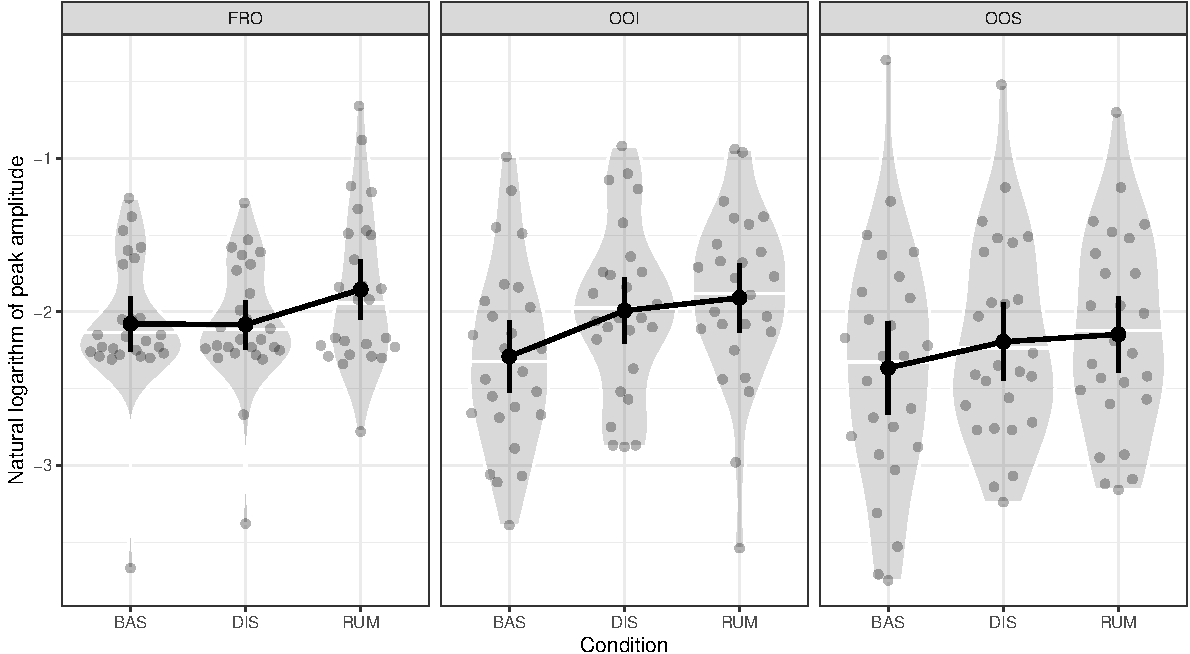
\includegraphics[width=1\linewidth]{manuscript_files/figure-latex/general-1} 

}

\caption{Average natural logarithm of the EMG peak amplitude per muscle and condition. The black dots and intervals represent the by-group average and 95\% confidence interval (N = 26). The horizontal white line in the violin plot represents the median. The grey dots represent the individual-level average natural logarithm of the EMG amplitude by muscle and condition.}\label{fig:general}
\end{figure}

\hypertarget{conclusions-from-under-powered-null-hypothesis-significance-tests}{%
\subsection{Conclusions from under-powered null-hypothesis significance tests}\label{conclusions-from-under-powered-null-hypothesis-significance-tests}}

There is an infamous tradition of conducting and interpreting uninformative null-hypothesis significance tests in Psychology (e.g., \protect\hyperlink{ref-meehl_appraising_1990-1}{Meehl, 1990a}, \protect\hyperlink{ref-meehl_theory-testing_1967}{1967}, \protect\hyperlink{ref-meehl_theoretical_1978}{1978}, \protect\hyperlink{ref-meehl_why_1990}{1990b}, \protect\hyperlink{ref-harlow_problem_1997}{1997}). By ``uninformative'', we mean that some null-hypothesis significance tests are simply not diagnostic with regards to the substantive effect of interest (e.g., whether there is a difference between conditions A and B).

As highlighted by several authors (e.g., \protect\hyperlink{ref-cohen_earth_1994}{J. Cohen, 1994}; \protect\hyperlink{ref-pollard_probability_1987}{Pollard \& Richardson, 1987}; \protect\hyperlink{ref-rouder_is_2016}{Rouder et al., 2016}), concluding that an effect is probably absent solely based on a non-significant \emph{p}-value is the continuous (i.e., probabilistic) extension of the modus tollens and is not a valid argument (i.e., the conclusion does not follow from the premises). This fallacious argument is also known as the \emph{fallacy of acceptance}, the \emph{absence of evidence fallacy} or \emph{the argument from ignorance}, and proceeds as follows: ``If the null hypothesis is true, then this observation should \emph{rarely} occur. This observation occurred. Therefore, the null hypothesis is false (or has low probability)''. In short, this argument is fallacious because it fails to consider the (probability of the data under the) alternative hypothesis.

This problem is tackled in modern usages of null-hypothesis significance tests by ensuring that the claim under scrutiny is submitted to \emph{severe} tests (e.g., \protect\hyperlink{ref-mayo_statistical_2018}{Mayo, 2018}; \protect\hyperlink{ref-mayo_severe_2006}{Mayo \& Spanos, 2006}). In general terms, the strong severity principle states that we have evidence for a claim to the extent that it survives a stringent scrutiny, that is, to the extent that it survives \emph{severe} tests. More precisely, some claim (e.g., \(\theta = 0\)) is said to be \emph{severely tested} if it had great chances of being corroborated/falsified, had the claim been true/false. When a statistical test is under-powered (for detecting a given effect size), the claim under scrutiny is not strongly (severely) tested, hence it not possible to obtain strong or reliable evidence for the claim (bad test, no evidence).

\hypertarget{optimistic-a-priori-power-analysis}{%
\subsection{Optimistic a priori power analysis}\label{optimistic-a-priori-power-analysis}}

Anticipating the legitimate critiques on the power of their study, Moffatt et al. (\protect\hyperlink{ref-moffatt_inner_2020}{2020}) report the results of a power analysis using the effect size reported in Nalborczyk et al. (\protect\hyperlink{ref-nalborczyk_orofacial_2017}{2017}) of \(d = 0.72\). This represents a highly optimistic estimate of the substantive effect of interest (i.e., the difference in the natural logarithm of the EMG peak amplitude between the rumination and distraction conditions) as this effect represents the standardised mean difference in EMG amplitude \emph{between a rest and a rumination periods} as estimated in Nalborczyk et al. (\protect\hyperlink{ref-nalborczyk_orofacial_2017}{2017}).

\begin{figure}[!htb]

{\centering 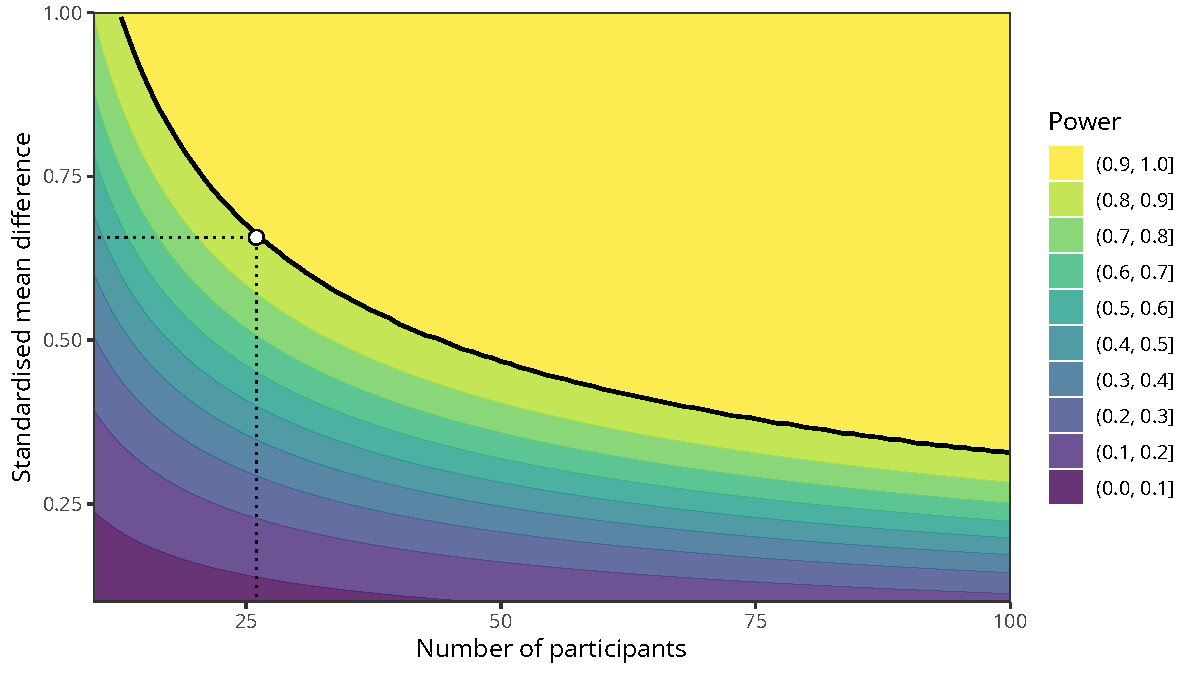
\includegraphics[width=1\linewidth]{manuscript_files/figure-latex/power-1} 

}

\caption{Statistical power as a function of both sample size and effect size, for a one-sample t-test with a significance level of 0.05. The white dot indicates the minimal effect size that can be detected with a probability equal or superior to 0.9 with a sample size of N = 26.}\label{fig:power}
\end{figure}

We suggest the (a priori) power of the study ran by Moffatt et al. (\protect\hyperlink{ref-moffatt_inner_2020}{2020}) was much lower than suggested by the authors. Indeed, we speculate that the standardised mean difference in EMG peak amplitude between the rumination and distraction conditions may be much weaker than the standardised mean difference in EMG amplitude between the rumination and rest conditions. If we assume that the former is half the size of the latter, therefore the a priori power of the main statistical test from Moffatt et al. (\protect\hyperlink{ref-moffatt_inner_2020}{2020}) was around \(0.42\), meaning that they had less than 1 chance out of 2 to find a significant effect (given that the population effect size was actually \(0.36\)). Notice that whereas taking half the effect size of Nalborczyk et al. (\protect\hyperlink{ref-nalborczyk_orofacial_2017}{2017}) may seem arbitrary, Figure \ref{fig:power} shows that a one-sample t-test with a sample size of \(N = 26\) is under-powered for a vast range of effect sizes.

\hypertarget{frequentist-properties-of-bayes-factors}{%
\subsection{Frequentist properties of Bayes factors}\label{frequentist-properties-of-bayes-factors}}

Once again, anticipating the legitimate critique that the absence of a significant difference is not necessarily ``significant'' evidence for the absence of an effect, Moffatt et al. (\protect\hyperlink{ref-moffatt_inner_2020}{2020}) reported the following Bayes factor (BF) analysis (p.12):

\begin{quote}
``{[}\ldots{]} therefore it is possible that the sample size of the present study lacked sufficient power to detect the effect of rumination on muscle activity. In order to test this, a Bayesian paired samples t-test was conducted for the peak log values of muscle activity between the rumination and distraction conditions. This revealed strong evidence in favour of the alternative hypothesis for the FRO muscle (\(B_{10} = 18.79\)), and moderate evidence in favour of the null hypothesis for the OOS (\(B_{10} = 0.232\)) and OOI (\(B_{10} = 0.278\)) muscles, according to current guidelines for interpreting Bayes factors {[}43{]}.''
\end{quote}

However, the current approach poses new problems. First, contrary to what the authors suggest, whereas computing a BF indeed allows assessing the \emph{relative evidence} for the null, computing a BF (i.e., comparing two models) does not solve the problem of low power. More precisely, the sensitivity (i.e., the ability to attain a certain goal) of an experimental design to detect a given effect is an issue for both frequentist and Bayesian statistical tests. To illustrate this point, we simulated 10.000 datasets (for \(N = 26\)) under the assumption of either no effect (i.e., the null hypothesis of \(d = 0\)), an effect size of \(d = 0.36\) (i.e., the supposed target effect size in \protect\hyperlink{ref-moffatt_inner_2020}{Moffatt et al., 2020}), or an effect size of \(d = 0.72\) (i.e., the effect size reported in \protect\hyperlink{ref-nalborczyk_orofacial_2017}{Nalborczyk et al., 2017}).

\begin{figure}[!htb]

{\centering 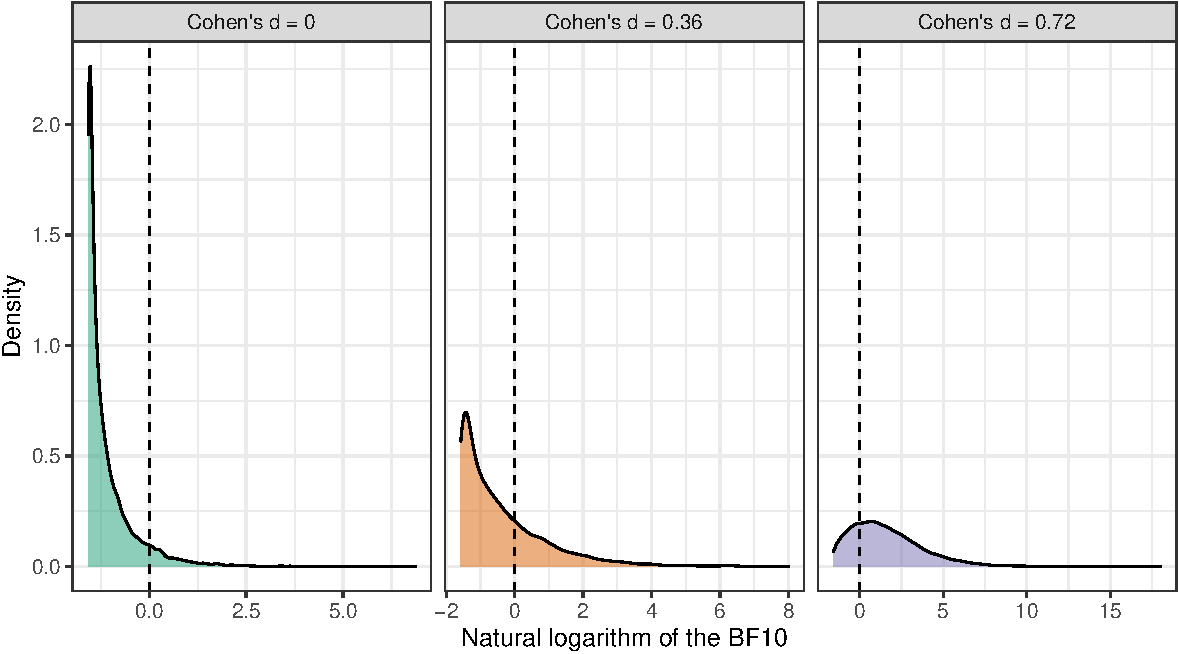
\includegraphics[width=1\linewidth]{manuscript_files/figure-latex/bf-dance-1} 

}

\caption{Illustrating the distribution of Bayes factors in favour of the alternative hypothesis for different population effect sizes (N = 26). In the left panel, the effect size is fixed to d = 0 (i.e., the null hypothesis), in the middle panel, it is fixed to d = 0.36 (i.e., the supposed target effect size in Moffatt et al., 2020), and in the right panel, the effect size is fixed to d = 0.72 (i.e., the effect size reported in Nalborczyk et al., 2017). The red vertical dashed line indicates the value of the BF computed for the OOI by Moffatt et al. (2020), on the logarithmic scale. The grey shaded area represents the conventional (but questionable) interval in which BFs are usually considered as inconclusive.}\label{fig:bf-dance}
\end{figure}

As shown in Figure \ref{fig:bf-dance}, the distribution of log-BFs computed under each hypothesis reveals important inter-simulation variability. For instance, 29.60\% of the computed log-BFs under the null hypothesis are ``inconclusive'' and 1.88\% of the log-BFs support the alternative hypothesis (although the population effect size is \(d = 0\)). When the population effect size is of \(d = 0.36\), 49.97\% of the computed log-BFs are ``inconclusive'' and 37.50\% of the log-BFs support the null hypothesis (although the population effect size is actually non-null). When the population effect size is of \(d = 0.72\), 41.65\% of the computed log-BFs are ``inconclusive'' and 6.41\% of the log-BFs support the null hypothesis. In brief, this simulations shows that for small sample and effect sizes, BFs have non-negligible error rates (see also \protect\hyperlink{ref-schonbrodt_sequential_2017}{Schönbrodt et al., 2017}).\footnote{It should be noted that, as stressed by Rouder (\protect\hyperlink{ref-rouder_optional_2014}{2014}), Bayes factors indicate the relative evidence for a hypothesis, conditional on some observed data. In other words, Bayesian updating is not conditional on some hypothetical truth. With this in mind, the present simulation aims at illustrating how the frequentist properties of BFs may be used to design more informative studies (see also \protect\hyperlink{ref-schonbrodt_bayes_2018}{Schönbrodt \& Wagenmakers, 2018}), while acknowledging that proper long-term error rates \emph{control} is not the realm of the Bayesian framework.}

The problems discussed above about the interpretation of under-powered non-significant results also apply to the test Moffatt et al. (\protect\hyperlink{ref-moffatt_inner_2020}{2020}) performed regarding the effect or the conditions' order. In Nalborczyk, Banjac, et al. (\protect\hyperlink{ref-nalborczyk_dissociating_2021}{2021}), we manipulated the modality of rumination (whether it is verbal or non-verbal) in a between-subject manner to avoid order effects and to avoid dissipating the effects of the negative mood induction. More precisely, we assumed that inducing rumination after a distraction condition in a within-subject manner would dissipate the effects of the mood induction and therefore reduce the impact of the rumination induction. In contrast to this approach, Moffatt et al. (\protect\hyperlink{ref-moffatt_inner_2020}{2020}) asked participants to ruminate and then distract themselves (or reciprocally), after an induced stressor (an induced failure). Anticipating again that the order of the within-subject conditions may be an issue, Moffatt et al. (\protect\hyperlink{ref-moffatt_inner_2020}{2020}) say:

\begin{quote}
``Unless otherwise reported, the inclusion of order in which the conditions were completed as a between-subjects variable as part of a mixed-design ANOVA produced no significant main effects or interactions involving order.'' (p.7)
\end{quote}

Unfortunately, obtaining a non-significant effect of the conditions' order is very weak evidence that order did not play a role in the results, given the low power of the tests that were performed (the sample size in each group was of N = 12 and N = 14).

\hypertarget{robustness-of-bayes-factors-to-prior-specifications}{%
\subsection{Robustness of Bayes factors to prior specifications}\label{robustness-of-bayes-factors-to-prior-specifications}}

Formulated in Bayesian terms, the problem of specifying credible effect sizes in a priori power analyses may be described as a problem of prior specification. However, defining sound prior distributions for the alternative hypothesis is notoriously difficult (for some guidance, see for instance \protect\hyperlink{ref-dienes_obtaining_2021}{Dienes, 2021}, \protect\hyperlink{ref-dienes_how_2019}{2019}). In Figure \ref{fig:sensitivity}, we report the results of prior \emph{sensitivity analyses}, depicting the value of the BF in favour of the alternative hypothesis (relative to the null hypothesis) for the difference between the distraction and rumination conditions, under various prior specifications, for each muscle.

\begin{figure}[!h]

{\centering 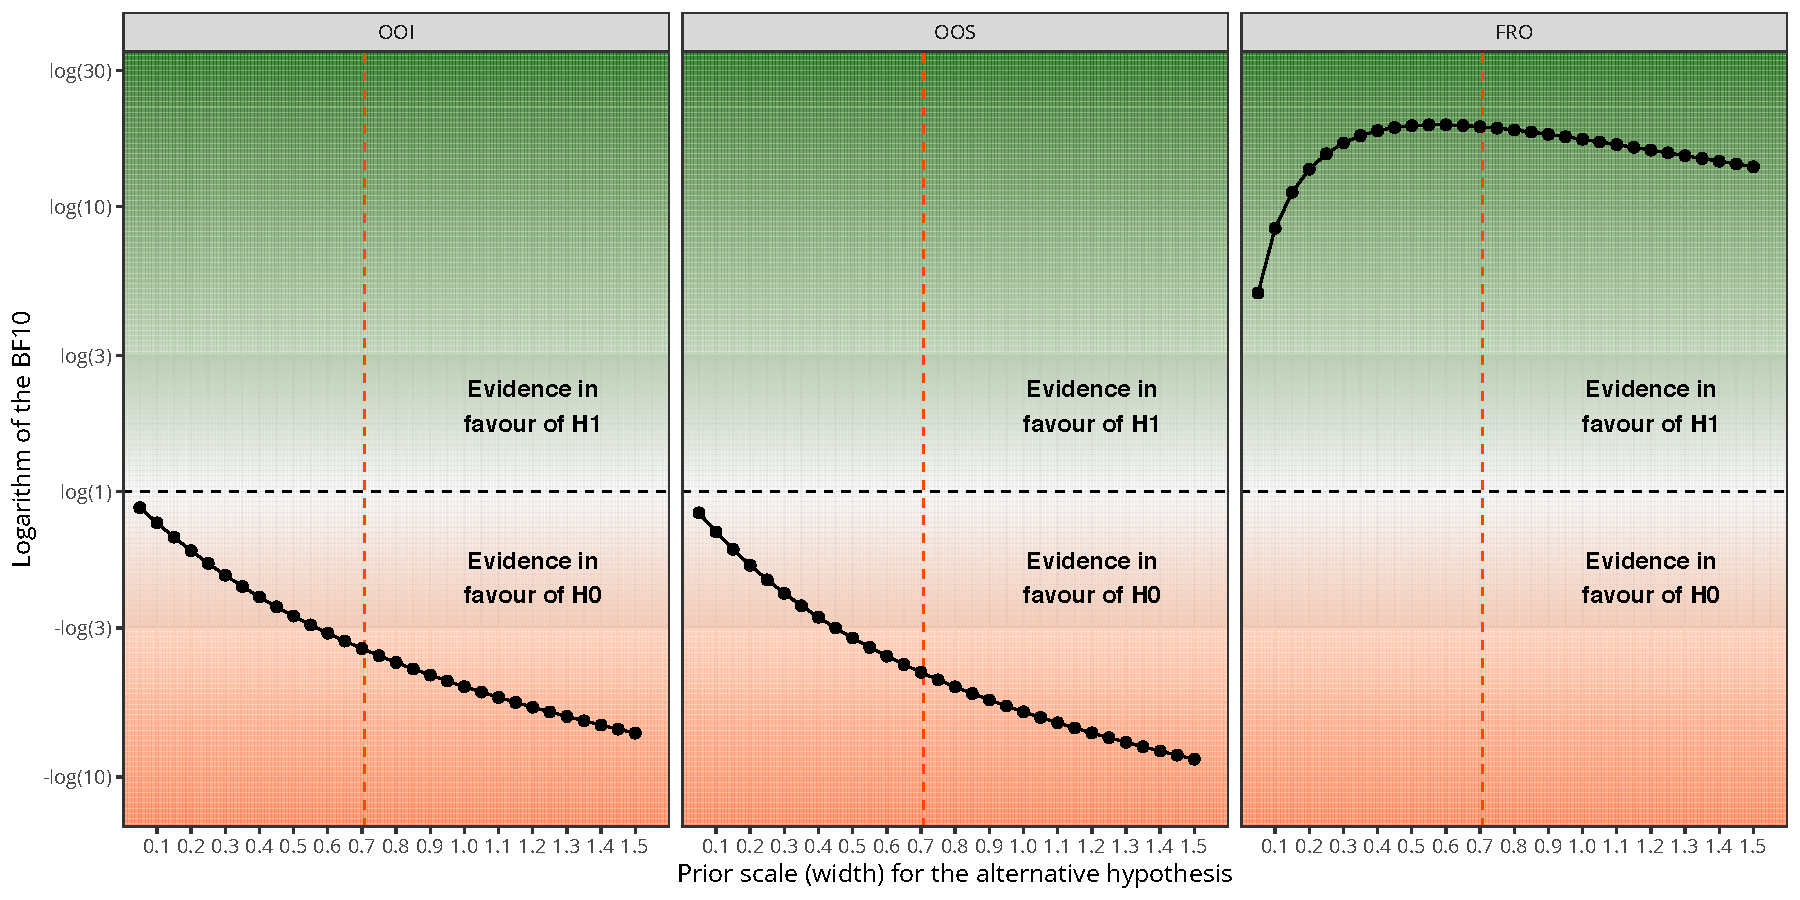
\includegraphics[width=1\linewidth]{manuscript_files/figure-latex/sensitivity-1} 

}

\caption{Prior sensitivity analysis for the Bayes factor computed for each muscle (OOI, OOS, and FRO). The x-axis represents the width of the prior put on the standardised effect size (i.e., the prior for the alternative hypothesis). The y-axis represents the logarithm of the Bayes factor in favour of the alternative hypothesis. The horizontal black dashed line represents equal support (evidence) for each hypothesis. The vertical red dashed line depicts the prior width used in Moffatt et al. (2020). The grey shaded area represents the conventional (but questionable) interval in which BFs are usually considered as inconclusive.}\label{fig:sensitivity}
\end{figure}

This figure strikingly reveals large variability in the resulting BF with various prior specifications. More precisely, when the scale (width) of the prior put on the standardised effect size is changed (along the x-axis), the BF changes accordingly. For instance, varying the prior scale from 0.1 to 1.0 for the OOI results in BFs from 0.78 to 0.21, respectively.

\hypertarget{discussion-and-conclusions}{%
\section{Discussion and conclusions}\label{discussion-and-conclusions}}

With this short paper, we aimed to nuance the strong conclusion made by Moffatt et al. (\protect\hyperlink{ref-moffatt_inner_2020}{2020}), who asserted that the inner experience of rumination was not related to its peripheral muscular correlates. First, we discussed the statistical and epistemological reasons that cast doubt upon the main conclusion of Moffatt et al. (\protect\hyperlink{ref-moffatt_inner_2020}{2020}). Because the statistical tests conducted by Moffatt et al. (\protect\hyperlink{ref-moffatt_inner_2020}{2020}) were heavily under-powered, they provide only weak evidence for an absence of difference between conditions. Second, we highlighted that the frequentist properties of Bayesian tools (e.g., Bayes factors) provide an important piece of information that may help design more informative studies. Third, sensitivity analyses further suggested that various prior specifications may lead to widely different Bayes factors.

In addition to these methodological limitations, we now wish to discuss the theoretical interpretations and implications of these results. As discussed in the introduction section, we previously conducted several studies aiming to assess the role of the speech motor system in rumination. Following our initial study (\protect\hyperlink{ref-nalborczyk_orofacial_2017}{Nalborczyk et al., 2017}), we ran an extension in which we compared verbal to non-verbal rumination. The results suggested that the facial EMG correlates of verbal and non-verbal rumination were similar (\protect\hyperlink{ref-nalborczyk_dissociating_2021}{Nalborczyk, Banjac, et al., 2021}). Given the ample evidence on the EMG correlates of inner speech production (for an overview, see Chapter 1 in \protect\hyperlink{ref-nalborczyk_understanding_2019}{Nalborczyk, 2019}), we needed to explain why this particular form of inner speech (induced rumination) was not associated with speech-specific peripheral muscular activity.

In Nalborczyk, Banjac, et al. (\protect\hyperlink{ref-nalborczyk_dissociating_2021}{2021}), we suggested that this observation was coherent with the mental-habit view of depressive rumination (\protect\hyperlink{ref-watkins_habit-goal_2014}{Watkins \& Nolen-Hoeksema, 2014}), which defines rumination as a habitual behaviour, automatically triggered by contextual cues such as negative mood. We know habitual behaviours are more automatic (i.e., they are not intentionally initiated) than non-habitual behaviours. Interestingly, it has been observed that the automaticity with which a verbal thought is evoked may influence the degree to which it is enacted, that is, the degree to which it recruits the speech motor system (e.g., \protect\hyperlink{ref-cohen_motor_1986}{B. H. Cohen, 1986}; \protect\hyperlink{ref-sokolov_inner_1972}{Sokolov, 1972}). According to B. H. Cohen (\protect\hyperlink{ref-cohen_motor_1986}{1986}), the presence of peripheral motor activity during inner speech production may be interpreted in terms of attention sharing. For instance, in novel (hence non-automatic) or difficult situations, the vividness of inner speech may be strengthened by increasing the speech motor activity, resulting in more salient auditory percepts. Relating this idea to the motor control framework we previously proposed (e.g., \protect\hyperlink{ref-grandchamp_condialint_2019}{Grandchamp et al., 2019}; \protect\hyperlink{ref-loevenbruck_cognitive_2018}{Lœvenbruck et al., 2018}), it may be said that the characteristics of the task or situation (e.g., novelty, difficulty) may influence the amount of inhibition that is applied to motor commands during inner speech production (\protect\hyperlink{ref-nalborczyk_role_2021}{Nalborczyk, Debarnot, et al., 2021}), hence resulting in more or less visible peripheral muscular activity (for a discussion of these ideas in the broader context of motor imagery, see \protect\hyperlink{ref-guillot_imagining_2012}{Guillot et al., 2012}).

Another possible interpretation is that automatic forms of inner speech may rely more heavily on higher-level (e.g., memory-based) cognitive processes whereas less automatic (i.e., more intentional or deliberate) forms of inner speech may rely more on simulation mechanisms via the use of internal models of the speech motor system (\protect\hyperlink{ref-nalborczyk_role_2021}{Nalborczyk, Debarnot, et al., 2021}; \protect\hyperlink{ref-nalborczyk_understanding_2019}{Nalborczyk, 2019}). In other words, the production of automatic versus non-automatic inner speech would be underpinned by different processes that would involve the speech motor system to a different extent. This distinction is similar to the distinction between the two routes of prediction-by-association and prediction-by-simulation in speech perception and comprehension (\protect\hyperlink{ref-pickering_integrated_2013}{Pickering \& Garrod, 2013}). The prediction-by-association mechanism would rely more on perceptual sensory experiences and domain-general cognitive abilities whereas the prediction-by-simulation mechanism would rely more on the simulation of the motor action leading to the speech auditory percept. In the former case, no peripheral muscular activity is expected, whereas in the latter case, the speech motor system would be involved in simulating or emulating the corresponding overt action (cf.~also the distinction between \emph{motor simulation} and \emph{direct simulation} in \protect\hyperlink{ref-tian_mental_2012}{Tian \& Poeppel, 2012}). Whether the physiological correlates of automatic versus non-automatic (deliberate) forms of inner speech differ because of inhibitory constraints or because they rely on different processes (e.g., prediction-by-association or prediction-by-simulation) remains an open empirical question. We previously discussed these issues in more length and suggested ways forward from an experimental perspective in the discussion of Nalborczyk (\protect\hyperlink{ref-nalborczyk_understanding_2019}{2019}).

To conclude, we wish to bring some nuance to the conclusion of Moffatt et al. (\protect\hyperlink{ref-moffatt_inner_2020}{2020}), who stated that ``In conclusion, induced rumination appeared to involve similar levels of inner speech-related muscle activity to a period of distraction'' (p.14). In consideration of the limitations discussed in the present article, this conclusion seems hasty. Indeed, we provided theoretical (epistemological) and empirical (via simulation and sensitivity analyses) reasons to doubt the strength of the evidence in favour of the null hypothesis in this study. This commentary stresses the importance of planning adequately-powered studies of induced rumination, and the need for more thoughtful statistical analyses and data interpretation, as recommended by Wasserstein et al. (\protect\hyperlink{ref-wasserstein_moving_2019}{2019}).

\hypertarget{acknowledgements}{%
\section*{Acknowledgements}\label{acknowledgements}}
\addcontentsline{toc}{section}{Acknowledgements}

We thank Antonio Schettino for suggesting to include the ``Dance of the Bayes factors'' simulation and for providing helpful comments on a previous version of this manuscript. We also thank Daniel Lakens and two anonymous reviewers for valuable comments on previous versions of this manuscript.

\hypertarget{funding-information}{%
\section{Funding information}\label{funding-information}}

This work, partly carried out within the Institut Convergence ILCB (ANR-16-CONV-0002), has benefited from support from the French government, managed by the French National Agency for Research (ANR) and the Excellence Initiative of Aix-Marseille University (A*MIDEX).

\hypertarget{supp}{%
\section{Data accessibility}\label{supp}}

The full code used to produce the manuscript, analyses, and figures, is available at \url{https://osf.io/ba3gk/}.

\hypertarget{competing-interests}{%
\section{Competing Interests}\label{competing-interests}}

The author has no competing interests to declare.

\hypertarget{references}{%
\section*{References}\label{references}}
\addcontentsline{toc}{section}{References}

\hypertarget{refs}{}
\begin{CSLReferences}{1}{0}
\leavevmode\vadjust pre{\hypertarget{ref-alderson-day_inner_2015}{}}%
Alderson-Day, B., \& Fernyhough, C. (2015). Inner speech: {Development}, cognitive functions, phenomenology, and neurobiology. \emph{Psychological Bulletin}, \emph{141}(5), 931--965. \url{https://doi.org/10.1037/bul0000021}

\leavevmode\vadjust pre{\hypertarget{ref-R-papaja}{}}%
Aust, F., \& Barth, M. (2017). \emph{{papaja}: {Create} {APA} manuscripts with {R Markdown}}. \url{https://github.com/crsh/papaja}

\leavevmode\vadjust pre{\hypertarget{ref-cohen_motor_1986}{}}%
Cohen, B. H. (1986). The motor theory of voluntary thinking. In R. J. Davidson, G. E. Schartz, \& D. Shapiro (Eds.), \emph{Consciousness and self-regulation}. Springer, Boston, MA.

\leavevmode\vadjust pre{\hypertarget{ref-cohen_earth_1994}{}}%
Cohen, J. (1994). The earth is round (p {\textless{}} .05). \emph{American Psychologist}, \emph{49}(12), 997--1003. \url{https://doi.org/10.1037/0003-066X.49.12.997}

\leavevmode\vadjust pre{\hypertarget{ref-dienes_obtaining_2021}{}}%
Dienes, Z. (2021). Obtaining {Evidence} for {No} {Effect}. \emph{Collabra: Psychology}, \emph{7}(1), 28202. \url{https://doi.org/10.1525/collabra.28202}

\leavevmode\vadjust pre{\hypertarget{ref-dienes_how_2019}{}}%
Dienes, Z. (2019). How {Do} {I} {Know} {What} {My} {Theory} {Predicts}? \emph{Advances in Methods and Practices in Psychological Science}, \emph{2}(4), 364--377. \url{https://doi.org/10.1177/2515245919876960}

\leavevmode\vadjust pre{\hypertarget{ref-ehring_repetitive_2008}{}}%
Ehring, T., \& Watkins, E. R. (2008). Repetitive negative thinking as a transdiagnostic process. \emph{International Journal of Cognitive Therapy}, \emph{1}(3), 192--205. \url{https://doi.org/10.1680/ijct.2008.1.3.192}

\leavevmode\vadjust pre{\hypertarget{ref-goldwin_concreteness_2012}{}}%
Goldwin, M., \& Behar, E. (2012). Concreteness of idiographic periods of worry and depressive rumination. \emph{Cognitive Therapy and Research}, \emph{36}(6), 840--846. \url{https://doi.org/10.1007/s10608-011-9428-1}

\leavevmode\vadjust pre{\hypertarget{ref-goldwin_concreteness_2013}{}}%
Goldwin, M., Behar, E., \& Sibrava, N. J. (2013). Concreteness of depressive rumination and trauma recall in individuals with elevated trait rumination and/or posttraumatic stress symptoms. \emph{Cognitive Therapy and Research}, \emph{37}(4), 680--689. \url{https://doi.org/10.1007/s10608-012-9507-y}

\leavevmode\vadjust pre{\hypertarget{ref-grandchamp_condialint_2019}{}}%
Grandchamp, R., Rapin, L., Perrone-Bertolotti, M., Pichat, C., Haldin, C., Cousin, E., Lachaux, J.-P., Dohen, M., Perrier, P., Garnier, M., Baciu, M., \& Lœvenbruck, H. (2019). The {ConDialInt} {Model}: {Condensation}, {Dialogality}, and {Intentionality} {Dimensions} of {Inner} {Speech} {Within} a {Hierarchical} {Predictive} {Control} {Framework}. \emph{Frontiers in Psychology}, \emph{10}. \url{https://doi.org/10.3389/fpsyg.2019.02019}

\leavevmode\vadjust pre{\hypertarget{ref-guillot_imagining_2012}{}}%
Guillot, A., Di Rienzo, F., MacIntyre, T., Moran, A., \& Collet, C. (2012). Imagining is not doing but involves specific motor commands: {A} review of experimental data related to motor inhibition. \emph{Frontiers in Human Neuroscience}, \emph{6}. \url{https://doi.org/10.3389/fnhum.2012.00247}

\leavevmode\vadjust pre{\hypertarget{ref-loevenbruck_cognitive_2018}{}}%
Lœvenbruck, H., Grandchamp, R., Rapin, L., Nalborczyk, L., Dohen, M., Perrier, P., Baciu, M., \& Perrone-Bertolotti, M. (2018). A cognitive neuroscience view of inner language: To predict and to hear, see, feel. In P. Langland-Hassan \& A. Vicente (Eds.), \emph{Inner speech: {New} voices} (p. 37). Oxford University Press.

\leavevmode\vadjust pre{\hypertarget{ref-Martin}{}}%
Martin, L. L., \& Tesser, A. (1996). Some ruminative thoughts. In R. S. Wyer (Ed.), \emph{Advances in social cognition, vol. 9} (Vol. 9, pp. 1--47). Hillsdale, NJ, US: Lawrence Erlbaum Associates, Inc.

\leavevmode\vadjust pre{\hypertarget{ref-R-wordcountaddin}{}}%
Marwick, B. (2019). \emph{Wordcountaddin: Word counts and readability statistics in r markdown documents}.

\leavevmode\vadjust pre{\hypertarget{ref-mayo_statistical_2018}{}}%
Mayo, D. G. (2018). \emph{Statistical {Inference} as {Severe} {Testing}: {How} to {Get} {Beyond} the {Statistics} {Wars}}. Cambridge University Press. \url{https://doi.org/10.1017/9781107286184}

\leavevmode\vadjust pre{\hypertarget{ref-mayo_severe_2006}{}}%
Mayo, D. G., \& Spanos, A. (2006). Severe {Testing} as a {Basic} {Concept} in a {Neyman}--{Pearson} {Philosophy} of {Induction}. \emph{The British Journal for the Philosophy of Science}, \emph{57}(2), 323--357. \url{https://doi.org/10.1093/bjps/axl003}

\leavevmode\vadjust pre{\hypertarget{ref-mclaughlin_effects_2007}{}}%
McLaughlin, K. A., Borkovec, T. D., \& Sibrava, N. J. (2007). The effects of worry and rumination on affect states and cognitive activity. \emph{Behavior Therapy}, \emph{38}(1), 23--38. \url{https://doi.org/10.1016/j.beth.2006.03.003}

\leavevmode\vadjust pre{\hypertarget{ref-meehl_appraising_1990-1}{}}%
Meehl, P. E. (1990a). Appraising and {Amending} {Theories}: {The} {Strategy} of {Lakatosian} {Defense} and {Two} {Principles} that {Warrant} {It}. \emph{Psychological Inquiry}, \emph{1}(2), 108--141. \url{https://doi.org/10.1207/s15327965pli0102_1}

\leavevmode\vadjust pre{\hypertarget{ref-meehl_theory-testing_1967}{}}%
Meehl, P. E. (1967). Theory-testing in {Psychology} and {Physics}: {A} methodological paradox. \emph{Philosophy of Science}, \emph{34}(2), 103--115. \url{https://doi.org/10.1086/288135}

\leavevmode\vadjust pre{\hypertarget{ref-meehl_theoretical_1978}{}}%
Meehl, P. E. (1978). Theoretical risks and tabular asterisks: {Sir} {Karl}, {Sir} {Ronald}, and the slow progress of soft psychology. \emph{Journal of Consulting and Clinical Psychology}, \emph{46}(4), 806--834. \url{https://doi.org/10.1037/0022-006X.46.4.806}

\leavevmode\vadjust pre{\hypertarget{ref-meehl_why_1990}{}}%
Meehl, P. E. (1990b). Why {Summaries} of {Research} on {Psychological} {Theories} are {Often} {Uninterpretable}. \emph{Psychological Reports}. \url{https://doi.org/10.2466/pr0.1990.66.1.195}

\leavevmode\vadjust pre{\hypertarget{ref-harlow_problem_1997}{}}%
Meehl, P. E. (1997). The problem is epistemology, not statistics: {Replace} significance tests by confidence intervals and quantify accuracy of risky numerical predictions. \emph{What If There Were No Significance Tests?}, 393--425. \url{http://citeseerx.ist.psu.edu/viewdoc/citations;jsessionid=72FF987997EFB5F0602B02E1A2E04E40?doi=10.1.1.693.9583}

\leavevmode\vadjust pre{\hypertarget{ref-moffatt_inner_2020}{}}%
Moffatt, J., Mitrenga, K. J., Alderson-Day, B., Moseley, P., \& Fernyhough, C. (2020). Inner experience differs in rumination and distraction without a change in electromyographical correlates of inner speech. \emph{PLOS ONE}, \emph{15}(9), e0238920. \url{https://doi.org/10.1371/journal.pone.0238920}

\leavevmode\vadjust pre{\hypertarget{ref-R-here}{}}%
Müller, K. (2017). \emph{Here: A simpler way to find your files}. \url{https://CRAN.R-project.org/package=here}

\leavevmode\vadjust pre{\hypertarget{ref-nalborczyk_understanding_2019}{}}%
Nalborczyk, L. (2019). \emph{Understanding rumination as a form of inner speech: Probing the role of motor processes} {[}\{PhD\} \{Thesis\}, Univ. Grenoble Alpes \& Ghent University{]}. \url{https://thesiscommons.org/p6dct/}

\leavevmode\vadjust pre{\hypertarget{ref-nalborczyk_dissociating_2021}{}}%
Nalborczyk, L., Banjac, S., Baeyens, C., Grandchamp, R., Koster, E. H. W., Perrone-Bertolotti, M., \& Lœvenbruck, H. (2021). Dissociating facial electromyographic correlates of visual and verbal induced rumination. \emph{International Journal of Psychophysiology}, \emph{159}, 23--36. \url{https://doi.org/10.1016/j.ijpsycho.2020.10.009}

\leavevmode\vadjust pre{\hypertarget{ref-nalborczyk_role_2021}{}}%
Nalborczyk, L., Debarnot, U., Longcamp, M., Guillot, A., \& Alario, F.-X. (2021). \emph{The role of motor inhibition during covert speech production} {[}Preprint{]}. PsyArXiv. \url{https://doi.org/10.31234/osf.io/3df57}

\leavevmode\vadjust pre{\hypertarget{ref-nalborczyk_orofacial_2017}{}}%
Nalborczyk, L., Perrone-Bertolotti, M., Baeyens, C., Grandchamp, R., Polosan, M., Spinelli, E., Koster, E. H. W., \& Lœvenbruck, H. (2017). Orofacial electromyographic correlates of induced verbal rumination. \emph{Biological Psychology}, \emph{127}, 53--63. \url{https://doi.org/10.1016/j.biopsycho.2017.04.013}

\leavevmode\vadjust pre{\hypertarget{ref-nalborczyk_articulatory_2022}{}}%
Nalborczyk, L., Perrone-Bertolotti, M., Baeyens, C., Grandchamp, R., Spinelli, E., Koster, E. H. W., \& Lœvenbruck, H. (2022). Articulatory {Suppression} {Effects} on {Induced} {Rumination}. \emph{Collabra: Psychology}, \emph{8}(1), 31051. \url{https://doi.org/10.1525/collabra.31051}

\leavevmode\vadjust pre{\hypertarget{ref-Nolen-Hoeksema2008}{}}%
Nolen-Hoeksema, S., Wisco, B. E., \& Lyubomirsky, S. (2008). Rethinking rumination. \emph{Perspectives on Psychological Science}, \emph{3}(5), 400--424. \url{https://doi.org/10.1111/j.1745-6924.2008.00088.x}

\leavevmode\vadjust pre{\hypertarget{ref-perrone-bertolotti_what_2014}{}}%
Perrone-Bertolotti, M., Rapin, L., Lachaux, J. P., Baciu, M., \& Lœvenbruck, H. (2014). What is that little voice inside my head? {Inner} speech phenomenology, its role in cognitive performance, and its relation to self-monitoring. \emph{Behavioural Brain Research}, \emph{261}, 220--239. \url{https://doi.org/10.1016/j.bbr.2013.12.034}

\leavevmode\vadjust pre{\hypertarget{ref-pickering_integrated_2013}{}}%
Pickering, M. J., \& Garrod, S. (2013). An integrated theory of language production and comprehension. \emph{Behavioral and Brain Sciences}, \emph{36}(04), 329--347. \url{https://doi.org/10.1017/S0140525X12001495}

\leavevmode\vadjust pre{\hypertarget{ref-pollard_probability_1987}{}}%
Pollard, P., \& Richardson, J. T. (1987). On the probability of making {Type} {I} errors. \emph{Psychological Bulletin}, \emph{102}(1), 159--163. \url{https://doi.org/10.1037/0033-2909.102.1.159}

\leavevmode\vadjust pre{\hypertarget{ref-R-base}{}}%
R Core Team. (2017). \emph{R: A language and environment for statistical computing}. R Foundation for Statistical Computing. \url{https://www.R-project.org/}

\leavevmode\vadjust pre{\hypertarget{ref-rouder_optional_2014}{}}%
Rouder, J. N. (2014). Optional stopping: {No} problem for {Bayesians}. \emph{Psychonomic Bulletin \& Review}, \emph{21}(2), 301--308. \url{https://doi.org/10.3758/s13423-014-0595-4}

\leavevmode\vadjust pre{\hypertarget{ref-rouder_is_2016}{}}%
Rouder, J. N., Morey, R. D., Verhagen, J., Province, J. M., \& Wagenmakers, E.-J. (2016). Is {There} a {Free} {Lunch} in {Inference}? \emph{Topics in Cognitive Science}, \emph{8}(3), 520--547. \url{https://doi.org/10.1111/tops.12214}

\leavevmode\vadjust pre{\hypertarget{ref-schonbrodt_bayes_2018}{}}%
Schönbrodt, F. D., \& Wagenmakers, E.-J. (2018). Bayes factor design analysis: {Planning} for compelling evidence. \emph{Psychonomic Bulletin \& Review}, \emph{25}(1), 128--142. \url{https://doi.org/10.3758/s13423-017-1230-y}

\leavevmode\vadjust pre{\hypertarget{ref-schonbrodt_sequential_2017}{}}%
Schönbrodt, F. D., Wagenmakers, E.-J., Zehetleitner, M., \& Perugini, M. (2017). Sequential hypothesis testing with {Bayes} factors: {Efficiently} testing mean differences. \emph{Psychological Methods}, \emph{22}(2), 322--339. \url{https://doi.org/10.1037/met0000061}

\leavevmode\vadjust pre{\hypertarget{ref-sokolov_inner_1972}{}}%
Sokolov, A. (1972). \emph{Inner speech and thought}. Springer-Verlag.

\leavevmode\vadjust pre{\hypertarget{ref-tian_mental_2012}{}}%
Tian, X., \& Poeppel, D. (2012). Mental imagery of speech: Linking motor and perceptual systems through internal simulation and estimation. \emph{Frontiers in Human Neuroscience}, \emph{6}. \url{https://doi.org/10.3389/fnhum.2012.00314}

\leavevmode\vadjust pre{\hypertarget{ref-wasserstein_moving_2019}{}}%
Wasserstein, R. L., Schirm, A. L., \& Lazar, N. A. (2019). Moving to a world beyond {`` \emph{p} {\textless{}} 0.05.''} \emph{The American Statistician}, \emph{73}(sup1), 1--19. \url{https://doi.org/10.1080/00031305.2019.1583913}

\leavevmode\vadjust pre{\hypertarget{ref-watkins_habit-goal_2014}{}}%
Watkins, E. R., \& Nolen-Hoeksema, S. (2014). A habit-goal framework of depressive rumination. \emph{Journal of Abnormal Psychology}, \emph{123}(1), 24--34. \url{https://doi.org/10.1037/a0035540}

\leavevmode\vadjust pre{\hypertarget{ref-R-tidyverse}{}}%
Wickham, H. (2017). \emph{Tidyverse: Easily install and load the 'tidyverse'}. \url{https://CRAN.R-project.org/package=tidyverse}

\leavevmode\vadjust pre{\hypertarget{ref-R-knitr}{}}%
Xie, Y. (2015). \emph{Dynamic documents with {R} and knitr} (2nd ed.). Chapman; Hall/CRC. \url{https://yihui.org/knitr/}

\leavevmode\vadjust pre{\hypertarget{ref-R-rmarkdown}{}}%
Xie, Y., Allaire, J. J., \& Grolemund, G. (2018). \emph{R markdown: The definitive guide}. Chapman; Hall/CRC. \url{https://bookdown.org/yihui/rmarkdown}

\end{CSLReferences}


\end{document}
